\documentclass[paper=a4, fontsize=11pt,twoside]{article}

% -------------------------------------------------------------------- 
% General Page Layout
% --------------------------------------------------------------------
\usepackage[a4paper]{geometry} 
\usepackage[parfill]{parskip}
\setlength{\oddsidemargin}{5mm}  % Remove 'twosided' indentation
\setlength{\evensidemargin}{5mm}

% --------------------------------------------------------------------
% Encoding and Language Settings
% --------------------------------------------------------------------
\usepackage[T1]{fontenc} 
\usepackage[utf8]{inputenc}   
% encoding may need to be changed depending on the system
\usepackage[swedish]{babel} 
\usepackage{lipsum} % Lorem Ipsum

% --------------------------------------------------------------------
%  Utilities (colors, links, pictures, ect...)
% --------------------------------------------------------------------
\usepackage{xcolor}
\usepackage{hyperref}
\usepackage{graphicx}
\usepackage{amssymb}
\usepackage{epstopdf}
\usepackage[round]{natbib}
\usepackage{float}
\usepackage{pgfplots}
\pgfplotsset{width=12cm,compat=1.9}
\usepackage{tikz}
\DeclareGraphicsRule{.tif}{png}{.png}{`convert #1 `dirname #1`/`basename #1 .tif`.png}

% -----------------------------------------------------------------------------%
% Title Page / Document Class Definitions (Please Don't Play With This)
% -----------------------------------------------------------------------------%
	
% Table of contents depth = section & subsection
\setcounter{tocdepth}{1}
																								
% Horizontal rule
\newcommand{\HRule}[1]{\rule{\linewidth}{#1}}   															
																											
% Document Number
\newcommand{\documentNumber}[1]{\centering PUSP1742#1 \\[1.0cm]}	 										
																											
% Document Version
\newcommand{\documentVersion}[1]{\centering \small{v.#1} \\[1.0cm]}

% Group Responsible
\newcommand{\documentResponsible}[1]{\centering  Ansvarig Grupp: #1}

% Document Creator Group
\newcommand{\documentCreator}[1]{\centering Uppgjord Av: #1}	 									
																										
% Title
\makeatletter \def\printtitle{ {\centering \@title\par}} \makeatother
																											
% Author .. not really used, but it can stay in case
\makeatletter \def\printauthor{ {\centering \large \@author}} \makeatother
																											
\newcommand{\grouptitlepage}[4]{ 
	\title{
		\documentNumber{#1}																						
		\documentVersion{#2}																				
		\HRule{0.5pt} \\ % Upper rule 
		\LARGE \textbf{\uppercase{#3}} \\
		\large \textbf{\uppercase{ETSF20 Grupp 2}} 
		\HRule{2pt} \\ [1.5cm]    
		\normalsize            
		\documentResponsible{#4} \\ 
		\documentCreator{#4}  
	}																							
	\maketitle																							
	\thispagestyle{empty} 																					
	\newpage 
}
% \grouptitlepage{doc number}{Version Number}{doc title}{group responsible for
% doc}
% --------------------------------------------------------------------------------%
% Title Page / Document Class Definitions (Please Don't Play With This)
% --------------------------------------------------------------------------------%


% \date{}                                            
% Activate to display a given date or keep commented for current date


% -------------------------------------------------------
% DOCUMENT START (YOU CAN IGNORE EVERYTHING ABOVE HERE)
% -------------------------------------------------------
\begin{document}

% -------------------------------------------------------
% Title Page START
% -------------------------------------------------------
\grouptitlepage
% the \# typesets a # character into the document, you will need to replace them
% in yourdocuments. This is a template, just plug in what you need between the
% {}s. Document Code Number (same as time reports)
{19}
% Document Version Number
{0.0}
% Document Title
{Projektslutrapport}
% Group Responsible For Document
{(PG) Projekt Grupp}
% -------------------------------------------------------
% Title Page END
% -------------------------------------------------------
\tableofcontents
% WRITE THINGS BELOW HERE

\section{Tidtabeller}
\begin{figure}[h]
\centering
\begin{tabular}{|l|c|c|c|c|c|}
\hline
\textbf{Dokument} & {\fontsize{8pt}{0.2cm}\selectfont Total} &
{\fontsize{8pt}{0.2cm}\selectfont Utveckling} &
{\fontsize{8pt}{0.2cm}\selectfont Informell Granskning} &
{\fontsize{8pt}{0.2cm}\selectfont Formell Granskning} &
{\fontsize{8pt}{0.2cm}\selectfont Omarbete}\\
\hline
SDP & 72.0 & 52.0 & 2.0 & 5.6 & 12.4\\
\hline
SRS & 138.3 & 111.6 & 8.5 & 6.0 & 12.3\\
\hline
SVVS & 54.5 & 36.7 & 5.2 & 7.2 & 5.5\\
\hline
STLDD & 224.0 & 205.4 & 7.2 & 5.6 & 6.0\\
\hline
SVVI & 38.3 & 29.9 & 5.0 & 1.4 & 2.0\\
\hline
SDDD & 129.3 & 129.3 & - & - & -\\
\hline
SVVR & 10.8 & 10.8 & - & - & -\\
\hline
SSD & 69.3 & 69.3 & - & - & -\\
\hline
PFR & 23.4 & 23.4 & - & - & -\\
\hline
\end{tabular}
\end{figure}

\begin{figure}[h]
\centering
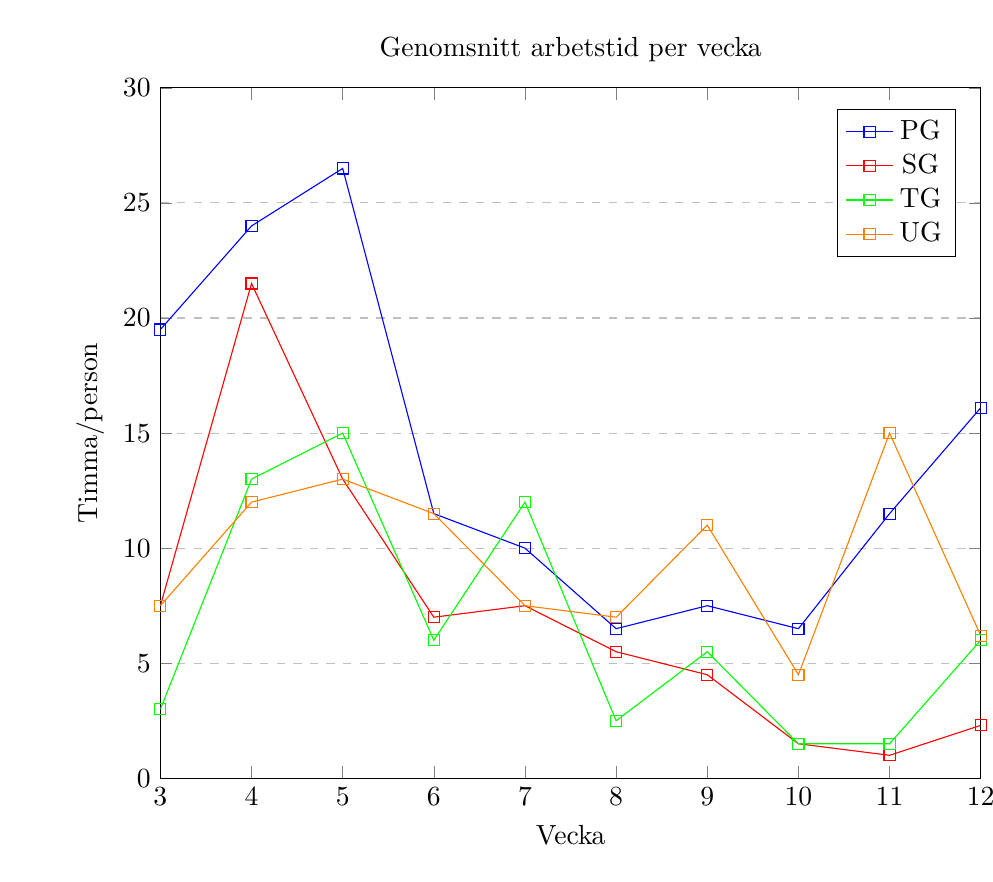
\begin{tikzpicture}
\begin{axis}[
    title={Genomsnitt arbetstid per vecka},
    xlabel={Vecka},
    ylabel={Timma/person},
    xmin=3, xmax=12,
    ymin=0, ymax=30,
    xtick={3,4,5,6,7,8,9,10,11,12},
    ytick={0,5,10,15,20,25,30},
    legend pos=north east,
    ymajorgrids=true,
    grid style=dashed,
]
%PG

\addplot[
    color=blue,
    mark=square,
    ]
    coordinates {
    (3,19.5)(4,24)(5,26.5)(6,11.5)(7,10)(8,6.5)(9,7.5)(10,6.5)(11,11.5)(12,16.1)
    };
%\addplot[color=blue]{14};

%SG 
\addplot[
    color=red,
    mark=square,
    ]
    coordinates {
    (3,7.5)(4,21.5)(5,13)(6,7)(7,7.5)(8,5.5)(9,4.5)(10,1.5)(11,1.0)(12,2.3)
    };
%\addplot[color=red]{7.2};

%TG
\addplot[
    color=green,
    mark=square,
    ]
    coordinates {
    (3,3)(4,13)(5,15)(6,6)(7,12)(8,2.5)(9,5.5)(10,1.5)(11,1.5)(12,6)
    };
%\addplot[color=green]{6.6};

%UG
\addplot[
    color=orange,
    mark=square,
    ]
    coordinates {
    (3,7.5)(4,12)(5,13)(6,11.5)(7,7.5)(8,7)(9,11)(10,4.5)(11,15)(12,6.2)
    };
%\addplot[color=orange]{10.1};
\legend{PG,SG,TG,UG}
 
\end{axis}
\end{tikzpicture}
\end{figure}

\begin{figure}[h]
\centering
\begin{tabular}{|l|c|c|c|c|c|c|c|c|c|c|c|}
\hline
{\fontsize{8pt}{0.2cm}\selectfont stil\_id} & {\fontsize{8pt}{0.2cm}\selectfont
total} & {\fontsize{8pt}{0.2cm}\selectfont v.3} &
{\fontsize{8pt}{0.2cm}\selectfont v.4} & {\fontsize{8pt}{0.2cm}\selectfont v.5}
& {\fontsize{8pt}{0.2cm}\selectfont v.6} & {\fontsize{8pt}{0.2cm}\selectfont v.7}
& {\fontsize{8pt}{0.2cm}\selectfont v.8} & {\fontsize{8pt}{0.2cm}\selectfont v.9}
& {\fontsize{8pt}{0.2cm}\selectfont v.10} & {\fontsize{8pt}{0.2cm}\selectfont
v.11} & {\fontsize{8pt}{0.2cm}\selectfont v.12} \\
\hline
dat13mde & 5485 & 720 & 1470 & 840 & 640 & 720 & 405 & 390 & 120 & 180 & - \\
\hline
dat14sfa & 8970 & 680 & 750 & 1265 & 760 & 510 & 575 & 1500 & 255 & 2475 & 200
\\
\hline
dat15bho & 4160 & 315 & 1210 & 885 & 345 & 360 & 420 & 330 & 90 & 145 & 60 \\
\hline
dat15cri & 3340 & 310 & 1150 & 590 & 285 & 285 & 165 & 120 & 45 & 45 & 345 \\
\hline
dat15csh & 5680 & 480 & 730 & 1065 & 765 & 645 & 525 & 420 & 150 & 450 & 450 \\
\hline
dat15jsu & 9065 & 365 & 940 & 750 & 1100 & 660 & 430 & 935 & 375 & 2640 & 870 \\
\hline
dat15mga & 3750 & 375 & 575 & 360 & 450 & 310 & 300 & 420 & 60 & 600 & 300 \\
\hline
dat15rel & 2425 & 360 & 405 & 420 & 410 & - & 300 & 430 & 100 & - & - \\
\hline
dat15sbe & 2970 & 345 & 445 & 525 & 330 & 330 & 300 & 270 & 240 & 185 & - \\
\hline
elt13spl & 2655 & - & 645 & 555 & 180 & 600 & 150 & 375 & 150 & - & - \\
\hline
fte11ama & 6630 & 710 & 965 & 1375 & 710 & 340 & 320 & 225 & 540 & 535 & 910 \\
\hline
gda10apo & 11367 & 450 & 1460 & 1222 & 1290 & 690 & 600 & 1740 & 255 & 2520 &
1140
\\
\hline
gin10ekr & 4520 & 295 & 1290 & 990 & 465 & 810 & 90 & 315 & 100 & - & 165 \\
\hline
mat13cgu & 4200 & 525 & 375 & 565 & 375 & 350 & 240 & 360 & 150 & 1260 & - \\
\hline
nat14ero & 4760 & 295 & 390 & 1120 & 455 & 755 & 210 & 320 & 55 & 250 & 910 \\
\hline
sas10gau & 10065 & 1635 & 1935 & 1790 & 660 & 840 & 470 & 640 & 245 & 825 &
1025 \\
\hline
\end{tabular}
\end{figure}

\end{document}










